\documentclass[12pt,twoside]{article}

% *** Set page dimensions ***
\raggedbottom
\parindent=0in
%\setlength{\topmargin}{-0.5in}
%\setlength{\oddsidemargin}{0.1875in}
%\setlength{\evensidemargin}{0in}
%\setlength{\textheight}{8.5in}
%\setlength{\textwidth}{6.225in}
%\addtolength{\oddsidemargin}{-0.7in}
%\addtolength{\evensidemargin}{-1.2in}
%\setlength{\oddsidemargin}{-0.2in}
%\setlength{\evensidemargin}{-0.2in}
%\addtolength{\textwidth}{1.4in}
%\addtolength{\topmargin}{-.875in}
%\addtolength{\textheight}{2.00in}

% *** Packages ***
\usepackage{alltt}
\usepackage{tocloft}
\usepackage{graphicx}
\usepackage{lscape}
\usepackage{amssymb}
\usepackage{float}
\usepackage{amsmath}
\usepackage{gensymb}
%\usepackage{subfigure}
\usepackage{lscape}
\usepackage{epsfig}
\usepackage{enumerate}
\usepackage{multicol}
\usepackage{fancyhdr}
\usepackage{epstopdf}
\usepackage{hyperref}
\usepackage{listings}

% *** Table of contents and Sectioning *** 
\setcounter{secnumdepth}{0}
\setcounter{tocdepth}{5}

% *** Table of contents and Sectioning *** 
\newcommand{\next}{\addtocounter{enumi}{9} \item}
\newcommand{\now}[1]{\setcounter{enumi}{#1}}
\newcommand{\Z}{\mbox{\sf Z\hspace{-1.5mm}Z}}
\newcommand{\R}{\mbox{\rm I\hspace{-0.75mm}R}}
\columnsep=0.75in

% *** Shortcuts for syntax ***
\newcommand{\ds}{\displaystyle }
\newcommand{\vsc}{\vspace{4mm}}
\newcommand{\dd}[1]{\frac{d}{d{#1}} \,} 
\newcommand{\ddx}{\frac{d}{dx} \,} 
\newcommand{\ddy}{\frac{d}{dy} \,} 
\newcommand{\ddz}{\frac{d}{dz} \,} 
\newcommand{\dydx}{\frac{dy}{dx} \,} 
\newcommand{\dydt}{\frac{dy}{dt} \,} 
\newcommand{\dfdx}{\frac{df}{dx} \,} 
\newcommand{\ddt}[1]{  \frac{d{#1}}{dt} }
\newcommand{\pp}[2]{  \frac{\partial{#1}}{\partial {#2}} }
\newcommand{\zx}{\frac{\partial z}{\partial x} \,}
\newcommand{\zy}{\frac{\partial z}{\partial y} \,}
\newcommand{\limh}{\lim_{h \rightarrow 0} \;}
\newcommand{\diff}{\frac{d}{dx} \,}
\newcommand{\de}{\Delta}
\renewcommand{\thesection}{\Roman{section}}
\newcommand{\bfr}{\begin{flushright}}
\newcommand{\efr}{\end{flushright}}
\newcommand{\dx}{\frac{\partial f}{\partial x} \,}
\newcommand{\dy}{\frac{\partial f}{\partial y} \,}
\newcommand{\p}{\partial}
\newcommand{\vi}{\vec{i}}
\newcommand{\vj}{\vec{j}}
\newcommand{\vk}{\vec{k}}
\newcommand{\lan}{\left\langle}
\newcommand{\ran}{\right\rangle}
\newcommand{\reading}[1] { {\em Reading: #1}}
\renewcommand{\Pr}{ \mbox{Pr}}

% *** Commands related to textbook references
\newcommand{\problem}{{\bf Problem.} }

% *** Footnoting with symbols ***
\long\def\symbolfootnote[#1]#2{\begingroup%
\def\thefootnote{\fnsymbol{footnote}}\footnote[#1]{#2}\endgroup}

% *** Defining a boxed note ***
\floatstyle{boxed}
\newfloat{noteinbox}{htb}{loa}
\newenvironment{boxnote}{\begin{noteinbox}[H]}{\end{noteinbox}}

\newcommand{\Question}{ {\bf Question: }  }
\newcommand{\Example}[1]{ {\bf Example: } {\em #1} }
\newcommand{\ExampleCont}[1]{ {\em #1} }

% *** Define the boxed Week #/summary at the beginning/end of every chapter ***
\newcommand{\sectionbox}[1]{% 
\begin{tabular}{|p{6in}|}%
\hline%
\ \\ %
{\Large {\bf {#1}}}  \\%
\ \\%
\hline%
\end{tabular}}

% *** Shortcuts *** 
\newcommand\goals{\large {\bf {Goals:}}}
\newcommand\setfont{ }

% *** Week commands: overwritten in each notes file
\newcommand{\Week}{Null-InPreambleCommon}
\newcommand{\WeekTitle}{Null-InPreambleCommon}
\newcommand{\Course}{MNTC P04}
\newcommand{\SetNum}{1 }
\newcommand{\topic}[1]{
\newpage
\setcounter{page}{1}
\fancyhead[LE,RO]{#1 - \thepage}
}

% *** Setup Latex for the large version of the files ***
%\usepackage[landscape]{geometry}
\usepackage[letterpaper,landscape,hmargin={.8in,.8in},vmargin={1in,0.2in}]{geometry}

% Remove paragraph indents
\setlength{\parindent}{0pt}

% Spacing at the top for the header is too large by default
\setlength{\voffset}{-5ex}

% **** RENEW SCALING COMMANDS HERE ****
% *** Text in boxes ***
\renewenvironment{boxnote}{\begin{noteinbox}[H] \huge}{\end{noteinbox}} 

% *** Chapter lead in/summary boxes ***
\renewcommand{\sectionbox}[1]{% 
\begin{tabular}{|p{9.5in}|}%
\hline%
\ \\ %
{\huge {\bf {#1}}}  \\%
\ \\%
\hline%
\end{tabular}}

% *** 'Section'' commands, which are sometimes used for spacing
% From http://zoonek.free.fr/LaTeX/LaTeX_samples_section/0.html
\makeatletter
 \renewcommand\section{\@startsection {section}{1}{\z@}%
                                    {-3.5ex \@plus -1ex \@minus -.2ex}%
                                    {0.3ex \@plus.2ex}%
                                    {\setfont\bf}}

 \renewcommand\subsection{\@startsection {subsection}{1}{\z@}%
                                    {-3.5ex \@plus -1ex \@minus -.2ex}%
                                    {0.3ex \@plus.2ex}%
                                    {\setfont\bf}}

% *** 'Goals' should be larger in the overheads ***
\renewcommand\goals{\huge {\bf {Goals:}}}
\renewcommand\setfont{\huge }

\thispagestyle{empty}

\setfont 

\newcommand{\WeekTitleOne}{Derivatives - Foundations}
\newcommand{\WeekTitleTwo}{Derivatives - Linearization and Applications}
\newcommand{\WeekTitleThree}{Derivatives - Modeling}
\newcommand{\WeekTitleFour}{Integrals - Foundations}
\newcommand{\WeekTitleFive}{Integrals - Techniques}
\newcommand{\WeekTitleSix}{Integrals - Modeling}
\newcommand{\WeekTitleSeven}{Differential Equations - }
\newcommand{\WeekTitleEight}{Differential Equations - }
\newcommand{\WeekTitleNine}{Differential Equations - }
\newcommand{\WeekTitleTen}{Linear Algebra - }
\newcommand{\WeekTitleEleven}{Linear Algebra - }
\newcommand{\WeekTitleTwelve}{Linear Algebra - }



\begin{document}
\setfont
\pagestyle{fancy}
\renewcommand{\Week}{2 }
\renewcommand{\WeekTitle}{\WeekTitleTwo }

\fancyhead[LE,RO]{Week \Week}  % default, usually only for first page
\fancyfoot{}
\sectionbox{Week \#\Week: \WeekTitle}


\vspace{5mm}
\goals
\begin{itemize}
\item Describe the meaning and value of linearization
\item Apply the technique of linearization to solve a variety of
  nonlinear equations
\item Use MATLAB to graph and compare functions with their
  linearizations
\item Use MATLAB to implement Newton's method
%\item Calculate and interpret the first and second derivatives, as
%  well as higher order derivatives
 \end{itemize}

\vspace{5mm}

\newpage
\topic{Linear Approximations}
\subsection*{Linear Approximations}

You should now feel comfortable in finding the derivative of a wide
variety of functions with formulas. \\[1ex]

In this section, we will explore how the derivatives you compute can
be tied back to understanding the behaviour of the original
function. \\[1ex]

We will start by returning to the definition of the derivative, based
on the $\ds \left(\frac{\mbox{rise}}{\mbox{run}}\right)$ formula for
slopes:
\begin{align*} 
  f'(x) = \frac{d}{dx} f = \dfdx = \lim_{\Delta x \to 0} \frac{\Delta f}{\Delta x} = \lim_{h \to 0} \frac{f(x+h) - f(x)}{h}
\end{align*} 



\newpage 
For example, if $y = f(x)$, then 
\[ \lim_{\Delta x \to 0} \frac{\Delta y}{\Delta x} = f'(x) 
\]
\begin{problem}
 What is the relationship between $f'$ and $\Delta y$,
	$\Delta x$ for merely {\em small} delta values? 
\end{problem}
\vfill

         Now sketch a graph, and label the two points
        in the $\Delta x$ difference `$x$' and `$a$'.  What expression
        do we obtain for $f(x)$?

        \vfill

\newpage
%We want to have a name for the RHS of this approximation:
\begin{boxnote}
\[ L(x)=f(a) + f'(a) (x-a) 
\]
\end{boxnote}
\begin{problem}
 What are some names for this linear function?
\end{problem}


 \newpage
 \problem Consider the tangent line approximation to the graph of
 $f(x)=e^x$ at $(0,1)$.  Find the formula for the tangent line at that
 point.

\vfill
\begin{minipage}[t]{0.4\linewidth}
\vspace{0pt}
  Sketch the graph of $y = e^x$ and the linearization/tangent line.
\end{minipage}
\hfill
\begin{minipage}[t]{0.45\linewidth}
\vspace{0pt}

\includegraphics[width=0.9\linewidth]{graphics/empty_graph_square_12}
\end{minipage}

% A good approximation for $e^{0.5}$ is therefore: \\[2ex]
% \begin{enumerate}[A.]
% \item $e^{0.5 }\approx 0.5$ \\[2ex]
% \item $e^{0.5 }\approx 1+e^{.5}$ \\[2ex]
% \item $e^{0.5 }\approx 1+.5$ \\[2ex]
% \end{enumerate}

% \end{problem}


\newpage

%\conques{%
% A function $f$ and its derivative have the following values at 0 and
% 10:%
% \begin{center}
% \begin{tabular}{cc}
% $f(0) = 2$ & $f(10) = 5$ \\
% $f^\prime (0) = -1$ & $f^\prime (10) = 1$
% \end{tabular}
% \end{center}
% Which of the following calculations produces the best estimate for
% $f(0.2)$?
% \begin{enumerate}
% \item[A. ] $(0.02)\times (5-2) + 2 = 2.06$
% \item[B. ] 2
% \item[C. ] $(0.2)\times (-1) = -0.2$
% \item[D. ] $(-1)\times (0.2) + 2 = 1.8$
% \end{enumerate}
% }%

\topic{Tangent Lines to Graphs}

\begin{problem}
Sketch the function $\ds f(x)=\frac{1}{x}$.
\end{problem}


\includegraphics[width=4in]{graphics/empty_graph_square_12}

\newpage

\begin{problem}
If we drew a tangent line to $f(x)$ at $x=4$, what range we would expect for the slope there?

\begin{enumerate}[A.]
\item Slope above 1. \\[2ex]
\item Slope between 0 and 1.  \\[2ex]
\item Slope between 0 and -1.\\[2ex] 
\item Slope below -1.
\end{enumerate}
\end{problem}



\newpage
\begin{problem}
 Find the linearization of $\ds f(x)=\frac{1}{x}$ at $a=4$.
\end{problem}
\vfill
\vfill

Find the equation of the tangent line to the function
$\ds y=\frac{1}{x} $ at $x=4$.  \vfill

\newpage

\problem Sketch the graph of $\ds y=\frac{1}{x}$, and its tangent line at $x=4$. 


\includegraphics[width=4in]{graphics/empty_graph_square_12}


\newpage
\topic{Linear Approximations for Error Estimation} Linear
approximations can be useful for quick and (relatively) simple error
calculations.

\begin{problem}
  A rock formation with high density ores was identified using gravity
  measurements; the formation is roughly cubic in shape. The edge each
  side of the cube was found to be 370 m, with a possible error in
  measurement of 10 m.  

  Use the ideas of linear approximations to estimate the maximum
  possible error (positive or negative) in computing the {\bf volume}
  of the formation.
\end{problem}
	\vfill
	\vfill

\newpage
\problem What are the trade-offs of using the linear approximation to
obtain the above error estimate, compared to a direct calculation of
the possible volumes with the error measurements?  \vfill


% \noindent \ques{Find the linearization of $f(x)=1/x$ at $a=4$.}
% %%%%% begin solution %%%%%%%%%%%%%%%%%%%%%%%%%%%%%%%%%%%%%%%%%%%
% \includesoln{\solntest}{\mbox{}\\[11cm]}{
% We can use our ``recipe'' to find the linearization of $f$:
% $$L(x)=f(a)+f'(a)(x-a)$$
% When $x=a$,
% \begin{align*}
% f(a) & = f(4)\\[0.1cm]
% & =\frac{1}{4}
% \end{align*}
% and
% \begin{align*}
% f'(a) & =-\frac{1}{a^2}\\[0.1cm]
% & = -\frac{1}{4^2}\\[0.1cm]
% & = -\frac{1}{16}
% \end{align*}
% So the linearization of $f(x)$ at $x=a$ is
% $$L(x)=\frac{1}{4}-\frac{1}{16}(x-4).\vi{1}$$}
% %%%%% end solution %%%%%%%%%%%%%%%%%%%%%%%%%%%%%%%%%%%%%%%%%%%%%
% \ques{Find the equation of the tangent line to the hyperbola $y=1/x$
% at $x=4$.}
% %%%%% begin solution %%%%%%%%%%%%%%%%%%%%%%%%%%%%%%%%%%%%%%%%%%%
% \includesoln{\solntest}{}{
% The tangent line of $y=\frac{1}{x}$ at $x=4$ and the line
% approximating the hyperbola $y=\frac{1}{x}$ at $x=4$ (linearization
% of the hyperbola) are the same line!  So using the previous example,
% we can write that the tangent line to the hyperbola at $x=4$ is
% $$y=\frac{1}{4}-\frac{1}{16}(x-4).$$}
%%%%% end solution %%%%%%%%%%%%%%%%%%%%%%%%%%%%%%%%%%%%%%%%%%%%%

\newpage
\topic{The $\sin(x)$ Approximation}
\subsection*{The $\sin(x)$ Approximation}
One of the most commonly-used approximation in physics
is the relationship
\[ \sin(x) \approx x
\]
\begin{problem}
 Derive this relationship using linearization. \vfill
\end{problem}

 What is the fine-print that should {\bf always} be associated with this approximation? \vspace{1in}

\newpage

\problem Sketch the graphs of $y = \sin(x) $ and $y = x$. \\
Focus on the domain $\ds \frac{-\pi}{2} \le x \le  \frac{\pi}{2}$.


\includegraphics[width=4in]{graphics/empty_graph_square_12}


\newpage  Below are more detailed calculations relating
$\sin(x)$ and $x$.  

\vspace{0.2in}

{\LARGE
	\begin{tabular}{||r||c|c|c|c|c|c|c|c||} \hline
	$x$ (degrees) &  & & & & & & & \\ \hline
	$x$ (rad) & 0.0500&          0.1000&          0.1500  & 0.2000  &0.2500 & 0.3000 & 0.3500 & 0.4000\\ \hline
	$\sin(x)$ & 0.0500 &0.0998 &0.1494 &0.1987 &0.2474 &0.2955 &0.3429 &0.3894 \\ \hline
	\end{tabular}
}\\[1ex]

\problem Comment on the agreement between $y=x$ and $y=\sin(x)$ on the range shown.

\vfill \vfill \vfill Most people are more familiar with angles
measured in degrees than radians: fill in the row indicating how many
degrees are represented by the radian measures.  \vfill

%\newpage

% Just for fun, put your calculator into degree mode, and see whether
% $\sin(x) \approx x$ still holds for small $x$.\\[1ex]

% \begin{tabular}{c|c}
%   $x$ (deg) & $\sin(x)$ \\ \hline
%   2$^o$ &  \\[2ex]
%   4$^o$ &  \\[2ex]
%   6$^o$  &  \\[2ex]
% \end{tabular}

\newpage

\topic{Linear Approximation In Beam Deflection}
\subsection*{Linear Approximation In Beam Deflection}

Sometimes engineering texts will use linear approximations without
explaining the source.  Here is a sample from a text on deflection of
beams under load.

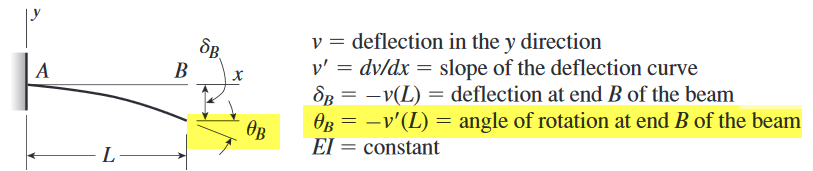
\includegraphics[width=0.95\linewidth]{graphics/notes_02_deflection}

\problem Compare the two meanings of $\theta_B$ highlighted.

\newpage

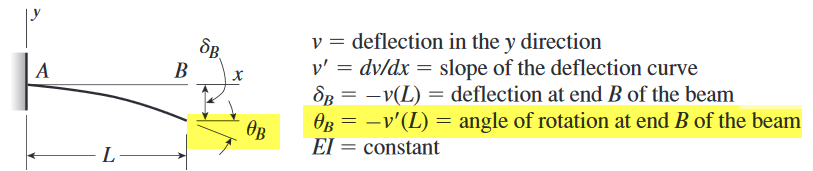
\includegraphics[width=0.95\linewidth]{graphics/notes_02_deflection}

\problem Use linearization to show that the slope at $L$ is
appromately equal to the angle of rotation.

\vfill

\newpage
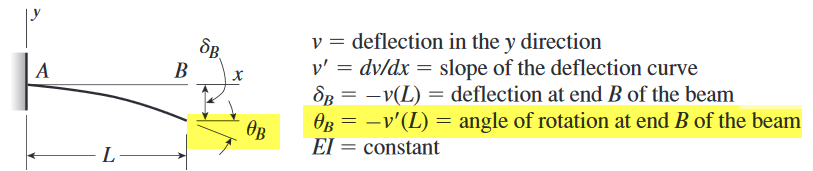
\includegraphics[width=0.95\linewidth]{graphics/notes_02_deflection}

$$ \mbox{slope} = \tan(\theta_B) \approx \theta_B$$

\problem As with any linear approximation, what is the fine print on this
relationship?

\vspace{1in}

Extra caution: what units would the angle $\theta_B$ have to be in for
this approximation to work?

\newpage
\topic{MATLAB Orientation}
\subsection*{MATLAB Orientation}

\vfill

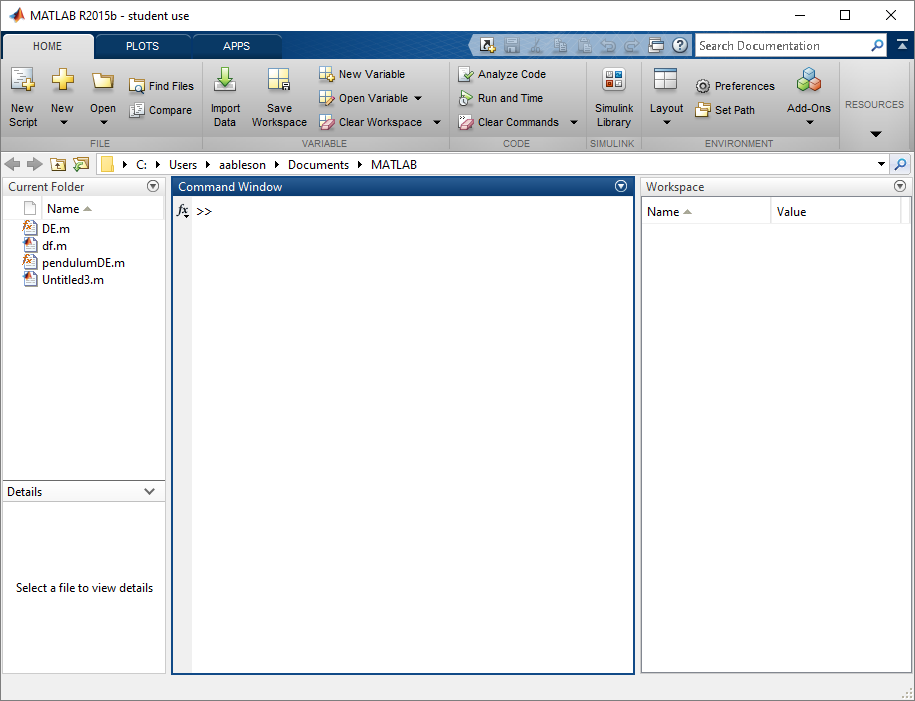
\includegraphics[width=0.8\linewidth]{graphics/notes_02_MATLAB_Windows}
\vfill

\newpage
\topic{MATLAB - Basic Commands}
\subsection*{MATLAB - Basic Commands}

{\bf Basic Usage:}
\begin{itemize}
\item Enter simple calculations at the
command prompt
\item Define variables at the command prompt
\item Use cursor keys to revisit previous
commands
\item Use first letters and cursor keys for more
control
\end{itemize}

\newpage
{\bf Scripts} 

Once you get past using single commands, you should store your program
in a `script', or M-file.
\begin{itemize}
\item File/New/Blank M-File, or
\item ��New Document�� button
\end{itemize}
You can run a script directly from the editor.
\begin{itemize}
\item F5, or
\item Press the ��Play�� button
\end{itemize}

\newpage
{\bf Further Commands}
\begin{itemize}
\item Standard mathematical functions are
built in:
\begin{itemize}
\item \texttt{cos, sin, log, log10, exp}
\end{itemize}
\item Suppress output with semi-colon
\item User variable names should be different from built-in functions,
  variables 
\item File/Clear Workspace (or type \texttt{clear}) to clear all
  variables
\end{itemize}

\newpage {\bf Matrices and MATLAB}

(Nearly) all MATLAB variables are matrices.
\begin{itemize}
\item scalars are \texttt{1x1} matrices
\item vectors are \texttt{1xn} or \texttt{nx1} matrices
\item  \texttt{size} function gives dimensions of a matrix
\end{itemize}
\newpage

{\bf Manually Creating Matrices}

Use square brackets to create matrices or vectors from list of numbers.
\begin{itemize}
\item \verb+v = [1 3 10]+
\end{itemize}
\vfill

Use colon notation to generate vectors by counting:
\begin{itemize}
\item \verb+w = 0:10+
\item \verb+z = 10:0.1:12+
\end{itemize}
\vfill

Use the \verb+linspace+ command to generate evenly-spaced values with
over a range.
\begin{itemize}
\item \verb+x = linspace(0, 4)+
\item \verb+x = linspace(0, 4, 10000)+
\end{itemize}

\topic{Graphing in MATLAB}
\subsection*{Graphing in MATLAB}

Basic syntax for generating a graph in MATLAB is:
\begin{verbatim}
close all
x = linspace(-2, 2);
y = exp(x);
plot(x, y)
\end{verbatim}

\newpage

{\bf Matrices and Graphing}

Try the following code to plot of a parabola
\begin{verbatim}
x = linspace(-2, 2)
y = x^2
plot(x, y)
\end{verbatim}
This is a very common issue when using MATLAB.

\verb+x^2+ means: \vfill

\verb+x.^2+ means: \vfill
\newpage
\topic{Tangent Lines in MATLAB}
\subsection*{Tangent Lines in MATLAB}

\problem Use MATLAB to graph the function $\ds y = \frac{1}{x}$, and
the tangent line to that graph at $x=4$.

\vfill

Useful new commands:
\begin{itemize}
\item \verb+hold on+ 
\item \verb+xlim([2, 5])+ 
\item \verb+ylim[[0, 1])+
\end{itemize}

\newpage

\problem Use MATLAB to graphically show the relationship between
$y = \tan(x)$ and its linear approximation $y = x$ for small $x$
values.



\newpage
\topic{Solving Non-Linear Equations}
\subsection*{Solving Non-Linear Equations}

One surprisingly challenging area of mathematics is back in
pre-calculus: simply solving equations with non-linear elements.

\problem Compare the difficulty in solving these two single-variable
equations.

Linear: $5 x = 10$ \vfill

Non-linear: $\ds e^x = x+5$ \vfill

\newpage

Some special types of non-linear equations {\bf can} be solved
algebraically.

\problem Find, by hand or with the help of a calculator, the solutions
to the following equations.

\[ x^2 + 2x + 3 = 0 \]
\vfill
\[ \log_{10}(x) = 3 \]
\vfill
\[ \sin(3x) = \cos(3x) \]
\vfill 
\newpage

Unfortunately, solving using algebra requires understanding how to
manipulate specific functions.  Worse yet, some equations can be
simply too complex to solve algebraically.

\problem Try to solve the following equations by hand: 
\[ \sin(3x) = x \]
\vfill
\[ xe^{-x} = 5 \]
\vfill

\newpage
\[ \sin(3x) = x \] 
\[ xe^{-x} = 5 \] 

In these more difficult cases, if we want a solution we must resort to
{\bf numerical methods}, which are all {\bf fancy versions of guess
  and check}!  This means numerical solutions are a poor second
choice, compared to by-hand solving:
\begin{itemize}
\item Numerical solutions give no insight into the solution
  (existence, patterns).
\item Numerical solving usually requires some amount of trial and
  error by the user.
\end{itemize}

\newpage

\topic{Example - Trajectories}
\subsection*{Example - Trajectories}
To generate a motivation for solving non-linear equations, we are
going to simulate the launch a motorcycle off the end of a ramp.  

\begin{center}
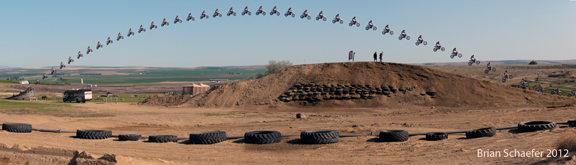
\includegraphics[width=0.7\linewidth]{graphics/notes_02_MotorcycleJump_2014} \\
Alex Harvill, age 19, lands 425 foot ramp-to-dirt record in May 2012.
\end{center}

The launch parameters are $v$, $\theta$, and $y_0$. \\
If you start with some basic physics equations, and break the
trajectory into components, you can arrive at the following formula:
\\ \vfill
$$ y= y_0 + \tan(\theta) ~x - \frac{1}{2} \frac{g}{\cos^2(\theta) (v)^2} ~x^2 $$


\newpage


\problem Write a MATLAB script that plots the trajectory of the
  motorcycle.  Use
\begin{itemize}
\item $y_0$ = 3 m, 
\item $v = 20$ m/s, and 
\item $\theta$ = 30 degrees.
\end{itemize}
Choose the $x$ interval so it shows the impact point.


\vfill

Add a horizontal line on the trajectory graph that shows the
  ground level, $y=0$.  Draw it in black.

\vfill

\newpage


\subsection*{Launch Angle - Ballistics}

Now consider the ballistics targeting problem, with practical
consequences on battlefields around the world.
\begin{center}
  Given the launch velocity, height, and a target $x$, what launch
  angle should be used?
\end{center}

\newpage 

\problem{Set $y_0 = 3$, and $v = 20$.  Experiment with the launch
  angle $\theta$ in MATLAB to find an angle that lands the motorcycle
  at $x=30$.}

\vfill

Comment on the simplicity and accuracy of this approach.

\newpage

\topic{Root-Finding vs Equation Solving}
\subsection*{Root-Finding vs Equation Solving}

In the ballistics example, it turns out to be very laborious, and
fairly inaccurate, to manually experiment with angles to find the
launch angle that will launch a projectile on to a target. We would
like to find a more systematic and robust approach.

\problem Express the targeting problem as a solution to a non-linear
equation.

\vfill

We will return to that example, but first we will consider the more
general challenge of solving non-linear equations, to give us a wider
context.

\newpage

Consider the following equations.
\begin{eqnarray*}
\mbox{Example 1: }\sin(x)  &  =  & \frac{1}{10} \ln(x) \\
\end{eqnarray*}
\begin{eqnarray*}
\mbox{Example 2: } x^5 - x^{10}   &  =  & e^{-x} \\
\end{eqnarray*}
Solving these equations as written involves balancing {\bf two}
functions, but life would be easier if we only had to deal with {\bf
  one}.

Rewrite each equation so that only one function is
  required.

\vfill

\newpage

{\bf Any} non-linear equation in the form $g(x) = h(x)$ can be written
as $f(x) = 0$ simply by moving all terms to the left side; the
solutions to both forms will be the same.  \\[1ex]

The $f(x) = 0$ form is preferable because:
\begin{itemize}
\item it only involves a single user-given function, and \\
\item all {\em non-linear equation solving} problems become {\em
    root-finding} problems.
\end{itemize}

\newpage

\topic{Newton's Method - Concept}
\subsection*{Newton's Method - Concept}

{\bf Concept:} If we are looking for the {\bf root of a non-linear
  function}, here is a reasonable search strategy.
\begin{itemize}
\item Find a reasonable starting point for our solution search, \\
  $x=a, y=f(a)$.
\item Imagine that $f(x)$ is approximately linear.
\item Find the tangent line to the function at $x=a$.
\item Find $c$, the root of the tangent line. 
  \begin{itemize}
  \item The new $x=c$ point should be closer to the real root of
    $f(x)$ than our original starting point, $x=a$.
  \end{itemize}
\end{itemize}

\newpage

{\bf Graphical Example} 

We want to find the $x$ values where the graph below crosses $y=0$.

\begin{itemize}
\item Suppose we start at initial starting point of $a = 4$.
\item Draw the tangent line at $x=a$, and follow it to its root,
  $x=c$.
\item Replace $a$ with the new point $c$.
\item Repeat the last two steps until $a$ and $c$ are almost the same,
  or don't change between iterations.
\end{itemize}
\begin{center}
  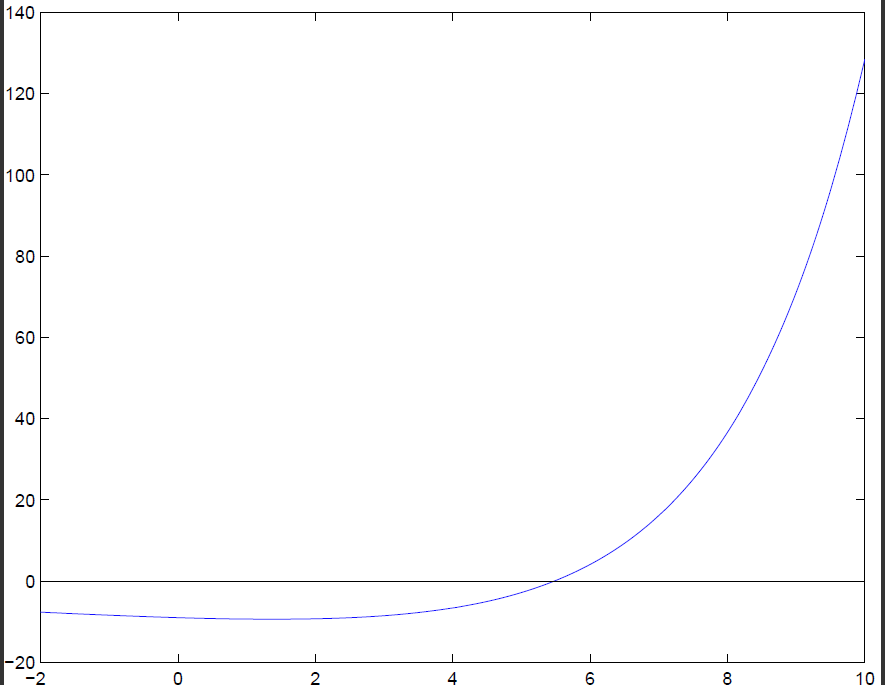
\includegraphics[width=0.4\linewidth]{graphics/notes_02_secant_example_graph}
\end{center}

\newpage

\begin{center}
  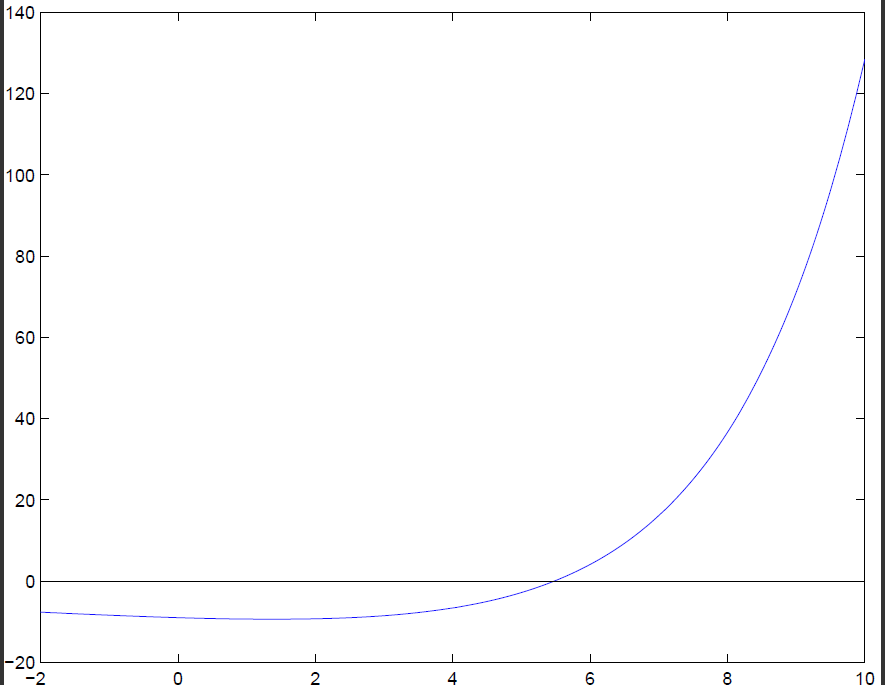
\includegraphics[width=7in]{graphics/notes_02_secant_example_graph}
\end{center}
\newpage
\begin{center}
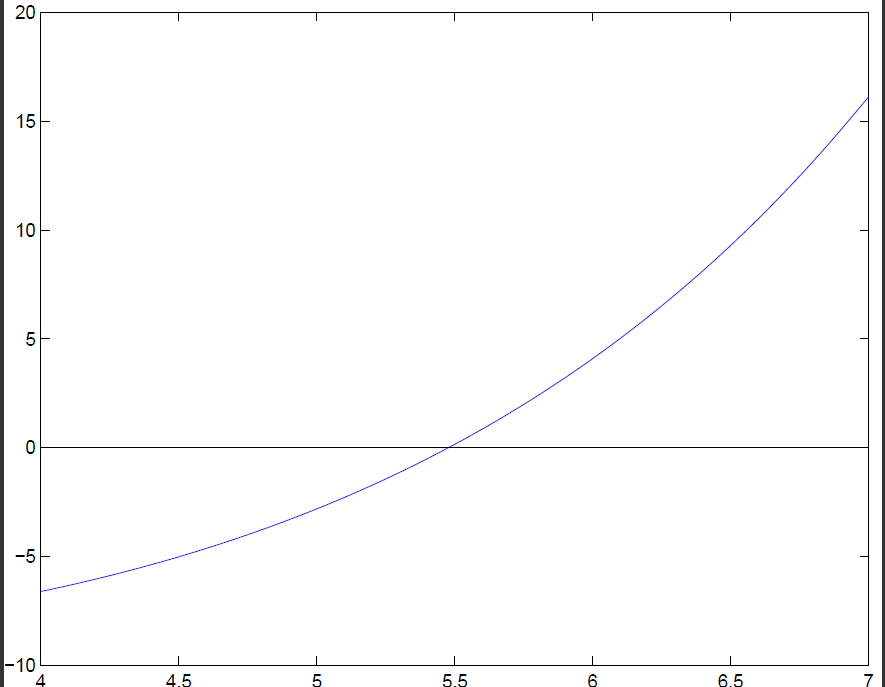
\includegraphics[width=7in]{graphics/notes_02_secant_example_graph_zoom}
\end{center}

\newpage

{\bf MATLAB Simulation}

\newpage

\topic{Newton's Method - Computational Algorithm}
\subsection*{Newton's Method - Computational Algorithm}

The two key steps of Newton's method are:
\begin{itemize}
\item Find the tangent line to the function at $x=a$.
\item Find $c$, the root of the tangent line. 
\end{itemize}
\problem How do we calculate the root of the tangent line to $f(x)$,
if the line is based on the point $x=a$?


\newpage

\problem In MATLAB, use Newton's method to find an approximation solution to
$$ e^{x/2} = x + 10$$

\vfill
\begin{center}
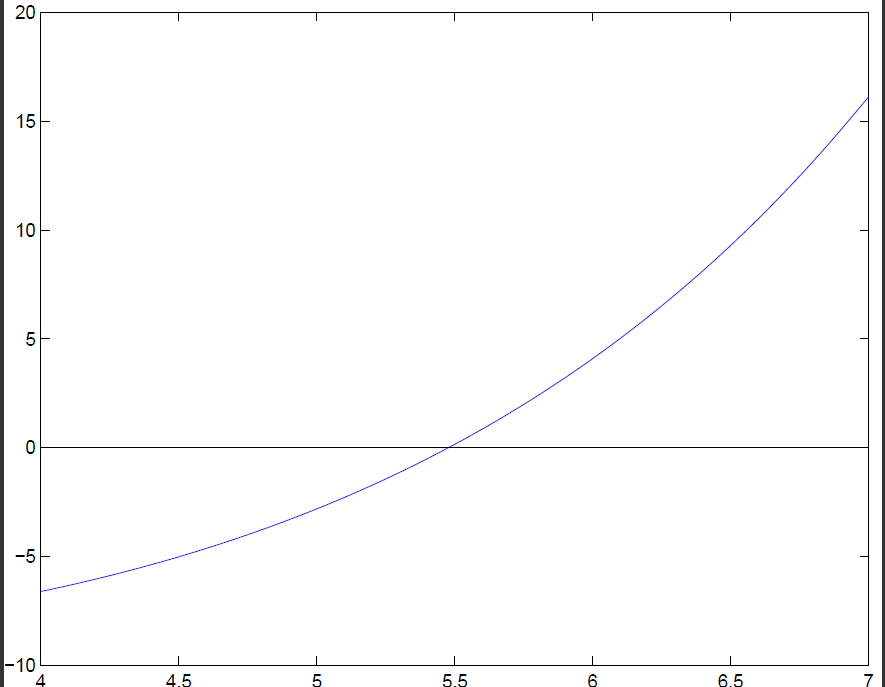
\includegraphics[width=4in]{graphics/notes_02_secant_example_graph_zoom} \\
Graph of $f(x) = e^{x/2}-x-10$
\end{center}


\newpage
\topic{Newton's Method - Trajectory Solution}
\subsection*{Newton's Method - Trajectory Solution}

\problem In MATLAB, use Newton's method to find the launch angle that
will land the a projectile at $x=30$, using the formula

$$ y = y_0 + \tan(\theta) ~x - \frac{1}{2} \frac{g}{\cos^2(\theta) (v)^2} ~x^2 $$
with $y_0 = 3$ m and $v = 20$ m/s.


\newpage


{\bf Comments} 

Newton's method is a sophisticated method for solving non-linear
equations. Some quick notes:
\begin{itemize}
\item The starting value of $x=a$ must be {\bf close to} the root (see
  practice problems).
  \begin{itemize}
  \item In practice, people will graph the function $f(x)$ to get a
    rough idea for where the roots might be. 
  \end{itemize}
\item Newton's method is vastly superior to using guess-and-check, or
  using loops, to find high-accuracy approximate solutions.
\end{itemize}


\end{document}

